\section{Nội dung thực hiện}

\begin{frame}{GIAO THỨC FRAME}
    \begin{figure}
    	\centering
    	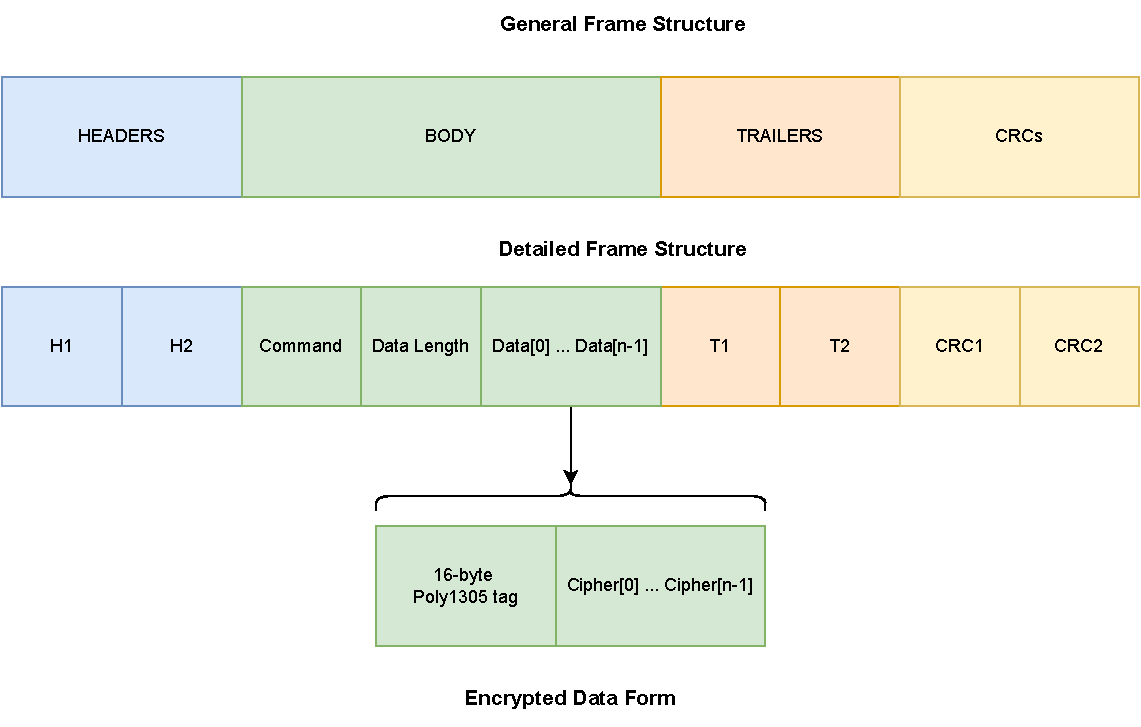
\includegraphics[width=1.0\textwidth,height=.8\textheight]{pic/Presentation-Page-2-Frame-Structure-Overview.pdf}
    \end{figure}
\end{frame}

\begin{frame}{CƠ CHẾ ĐỒNG BỘ}
    \begin{figure}
    	\centering
    	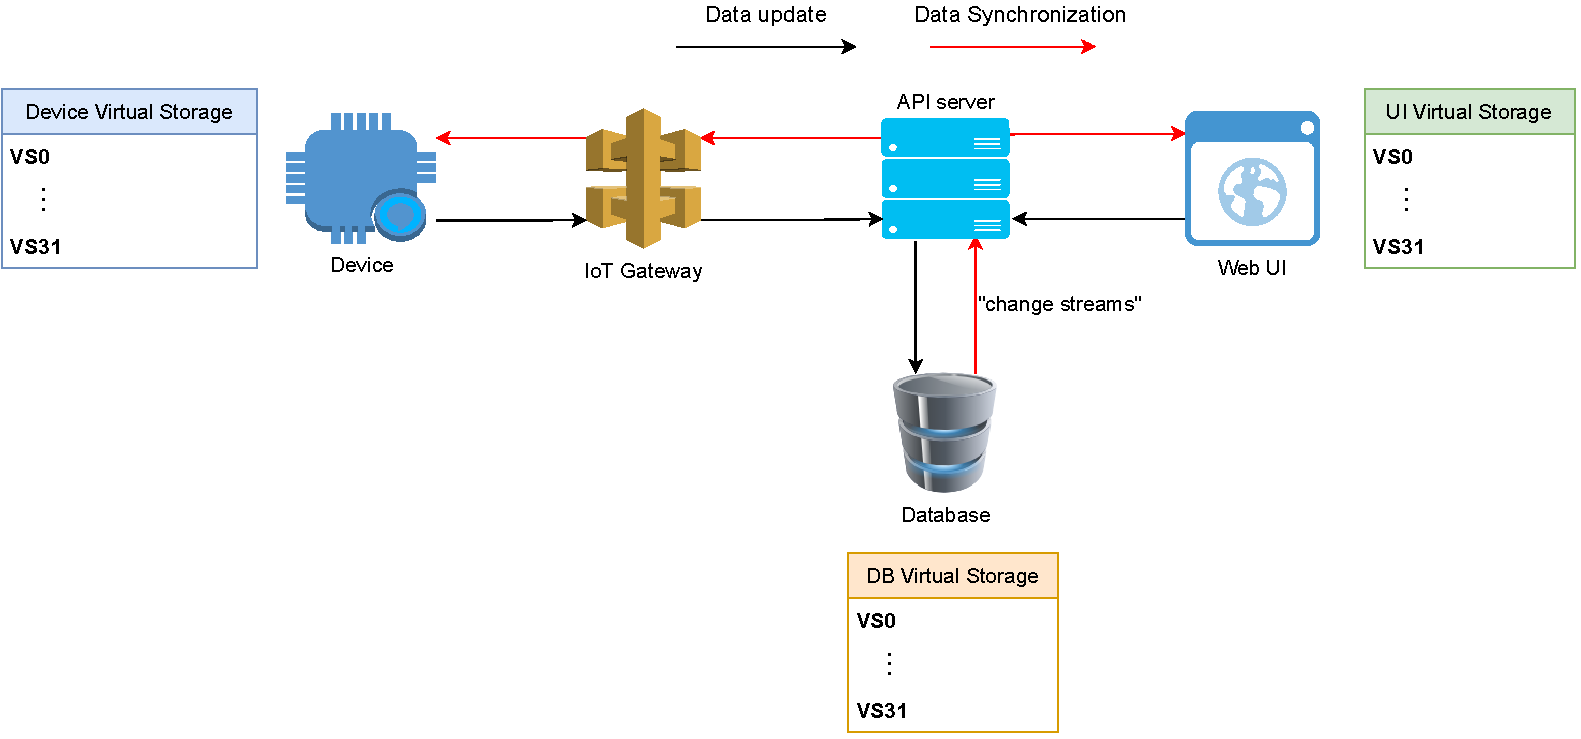
\includegraphics[width=1.0\textwidth]{pic/Presentation-Page-3-sync-mecha.pdf}
    \end{figure}
\end{frame}

\begin{frame}{GIAO DIỆN WEB LINH HOẠT}
    \begin{figure}
    	\centering
    	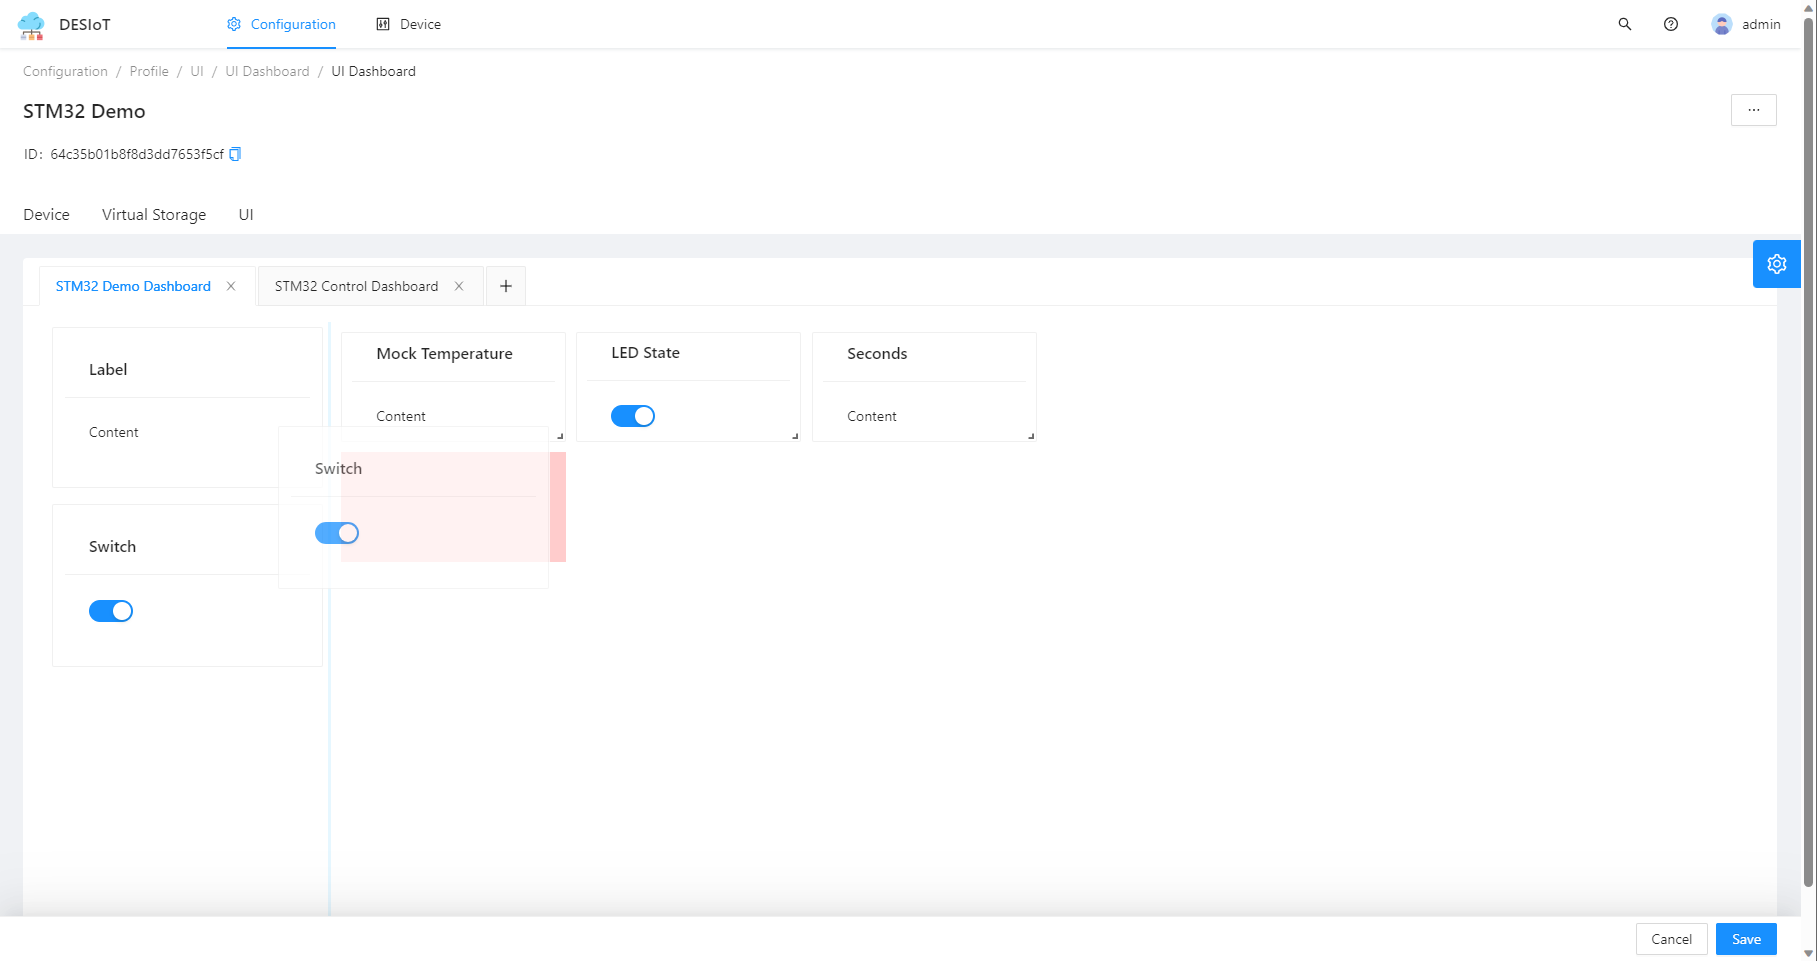
\includegraphics[width=1.0\textwidth,height=0.8\textheight]{pic/fig-config-ui-tab-edit-mode.png}
    \end{figure}
\end{frame}

\begin{frame}{BO MẠCH VÀ HỆ THỐNG BACK-END}
\begin{figure}
	\centering
	\subfigure
	{
		\begin{minipage}{0.2\linewidth}
    		\begin{figure}
    			\centering
    			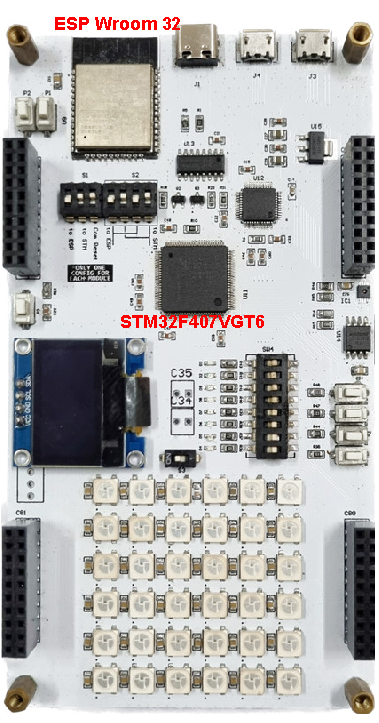
\includegraphics[scale=0.5]{pic/Presentation-Page-4-Bo-mach.pdf}
    		\end{figure}
    	\end{minipage}
	}
	\subfigure
	{
		\begin{minipage}{0.7\linewidth}
    		\begin{figure}
				\raggedleft
    			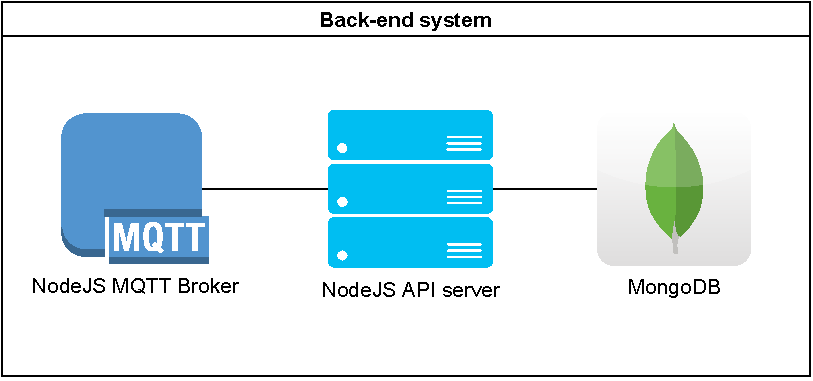
\includegraphics[scale=.6]{pic/Presentation-Page-5-Back-end-system.pdf}
    		\end{figure}
    	\end{minipage}
	}
\end{figure}
\end{frame}

\begin{frame}{MẬT MÃ HÓA CHACHA20-POLY1305}
	Sự kết hợp của thuật toán mã hóa dòng ChaCha20 và xác thực tin nhắn Poly1305.

	\begin{figure}
		\subfigure
		{
		\begin{minipage}{0.3\linewidth}
    		\begin{figure}
    			\raggedright
    			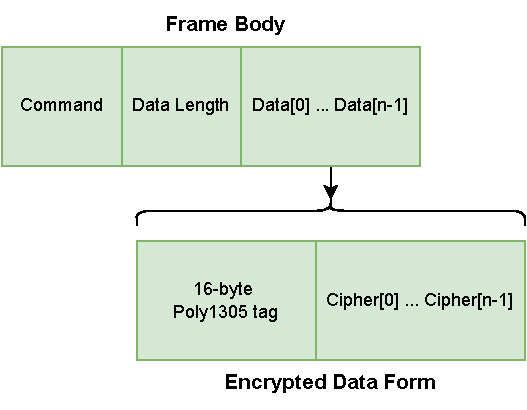
\includegraphics[scale=0.5]{pic/Presentation-Page-10-Frame-Body-Encrypt-Structure.pdf}
    		\end{figure}
    	\end{minipage}
		}
		\subfigure
		{
		\begin{minipage}{0.6\linewidth}
    		\begin{figure}
    			\hspace*{.5cm}
				\raggedright
    			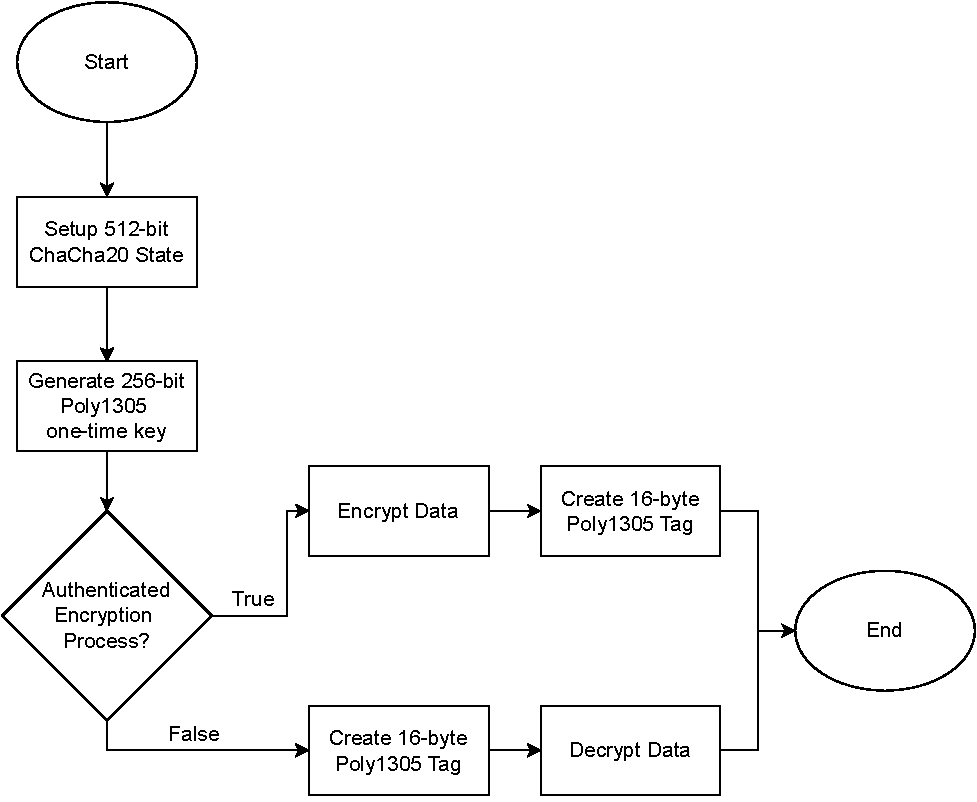
\includegraphics[width=1.0\textwidth,height=.7\textheight]{pic/Presentation-Page-9-CC20-P1305-Process.pdf}
    		\end{figure}
    	\end{minipage}
		}
	\end{figure}
\end{frame}
